% !TEX root = Eco-Model.tex
\section{Background} % (fold)
\label{sec:background}

As an application of networked manufacturing, cloud manufacturing proposed by ...

(problems background to form the ecosystem)

\subsection{Cloud manufacturing ecosystem} % (fold)
\label{sub:cloud_manufacturing_ecosystem}

\subsubsection{Cloud manufacturing ecosystem architecture}

Combined with the background of the research problem and other scholars' previous study in cloud manufacturing, we proposed an improved framework that suits for cloud manufacturing environment as shown in \autoref{fig:structure}.
\begin{figure}[htbp]
\centering
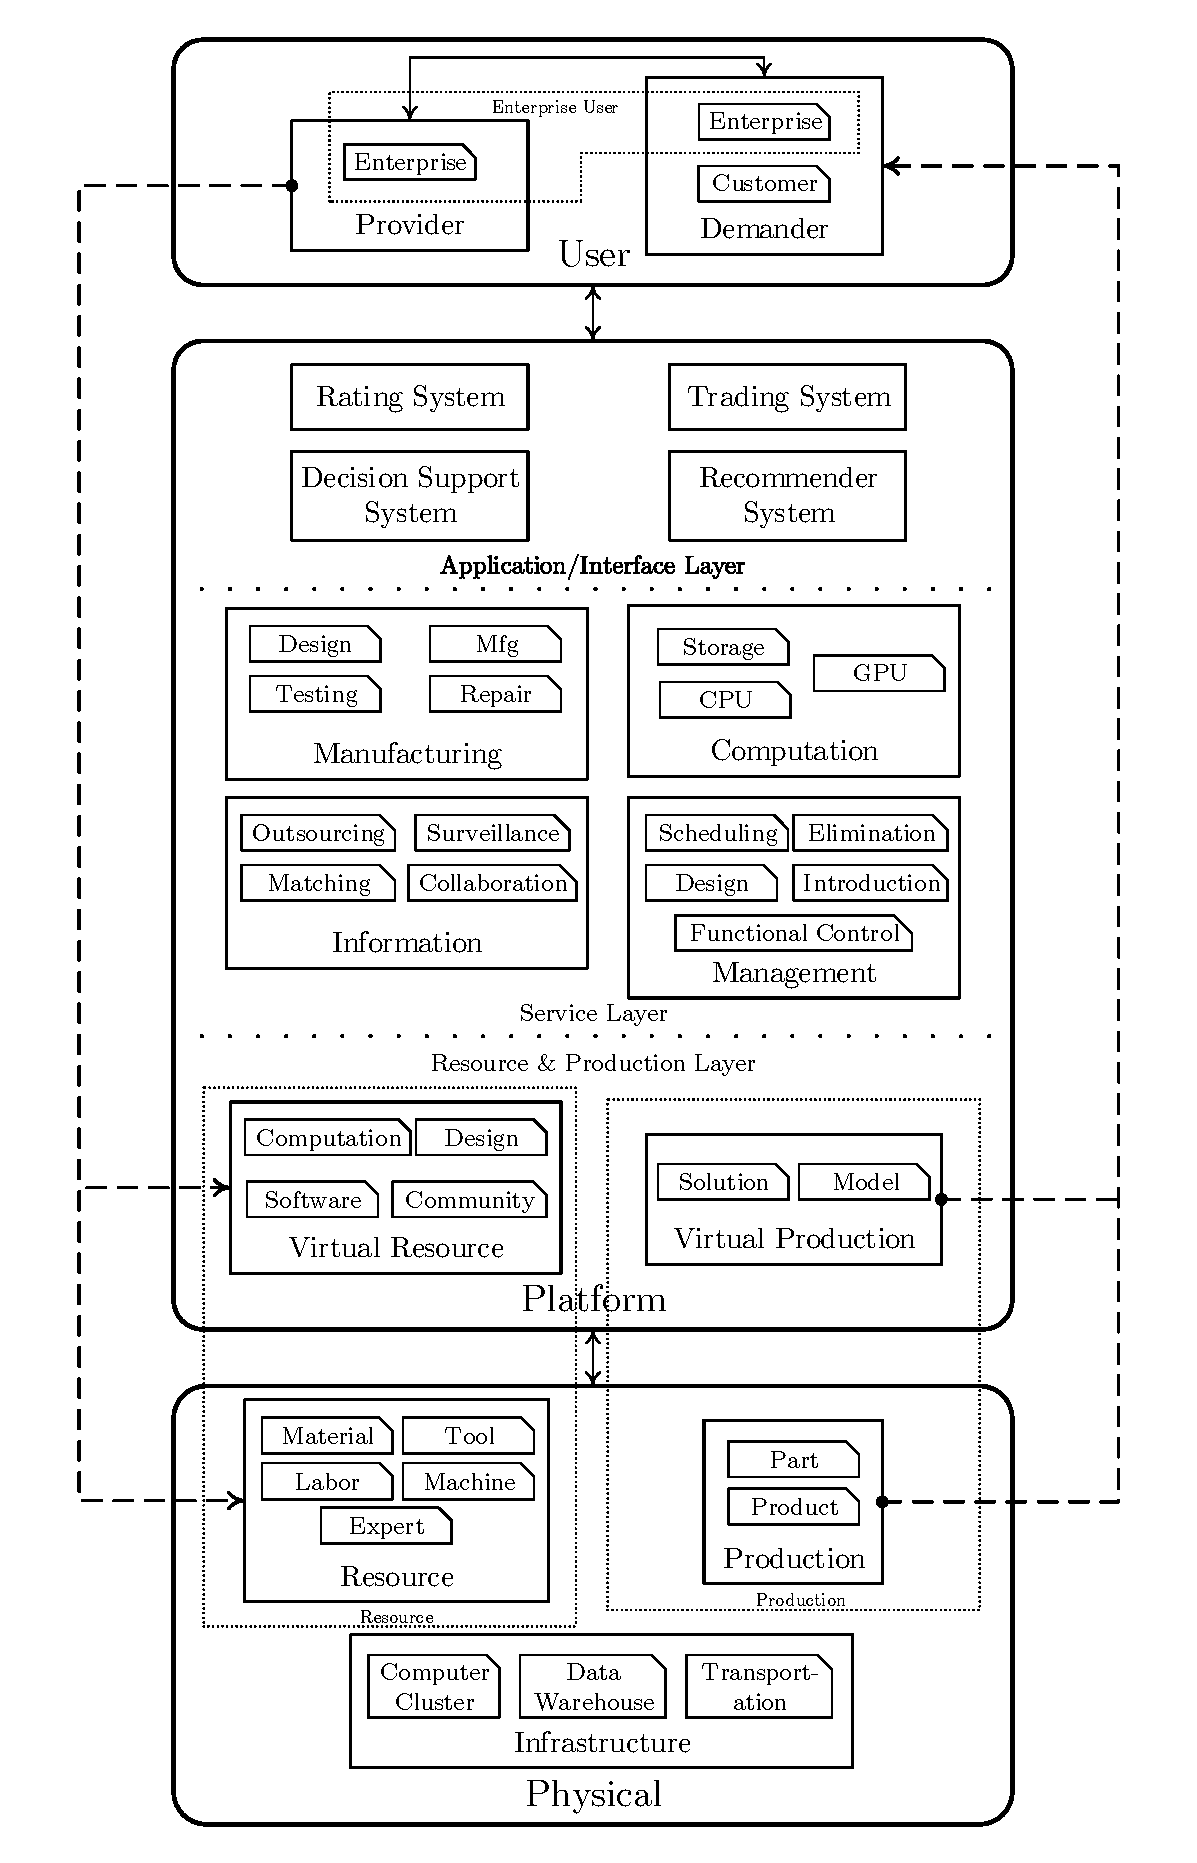
\includegraphics[scale = .6, trim = 0 15 0 35]{Cloud_Mfg_Structure.pdf}
\caption{Cloud manufacturing architecture with main flows}
\label{fig:structure}
\end{figure}

The architecture of cloud manufacturing is mainly composed of three parts, namely, \begin{inparaenum}[1)]
\item user,
\item platform and
\item physical base
\end{inparaenum}, that are connected by material or information flows. A simple version of conception for cloud manufacturing architecture we study here can be described as follows:
\begin{compactdesc}
\item [User] part describes the main roles in the cloud manufacturing environment like manufacturing service provider and manufacturing service demander, whome can be called as provider and demander for short respectively, from the functional point of view. Meanwhile, these roles can also be classified into enterprise user and customer, from the practical point of view. Both functional and practical are important perspective for later analysis in following sections. 
\item [Platform] part consists of 3 main layers namely
	\begin{inparaenum}[1)]
	\item application/interface layer,
	\item service layer and 
	\item resource \& production layer
	\end{inparaenum}.
Service is the core concept in cloud manufacturing, so service layer is the core in the cloud manufacturing platform. With the help of related technology in servitization, manufacturing resource and production can be encapsulated into services, then these services can be acquired by users with the well designed applications or interfaces.
\item [Physical Base] part includes the basic infrastructure, resource and production. It's worth mentioning that part of resources and production can even be virtualized with some services the platform provides.
\end{compactdesc}
 
\begin{figure}[htbp]
\centering
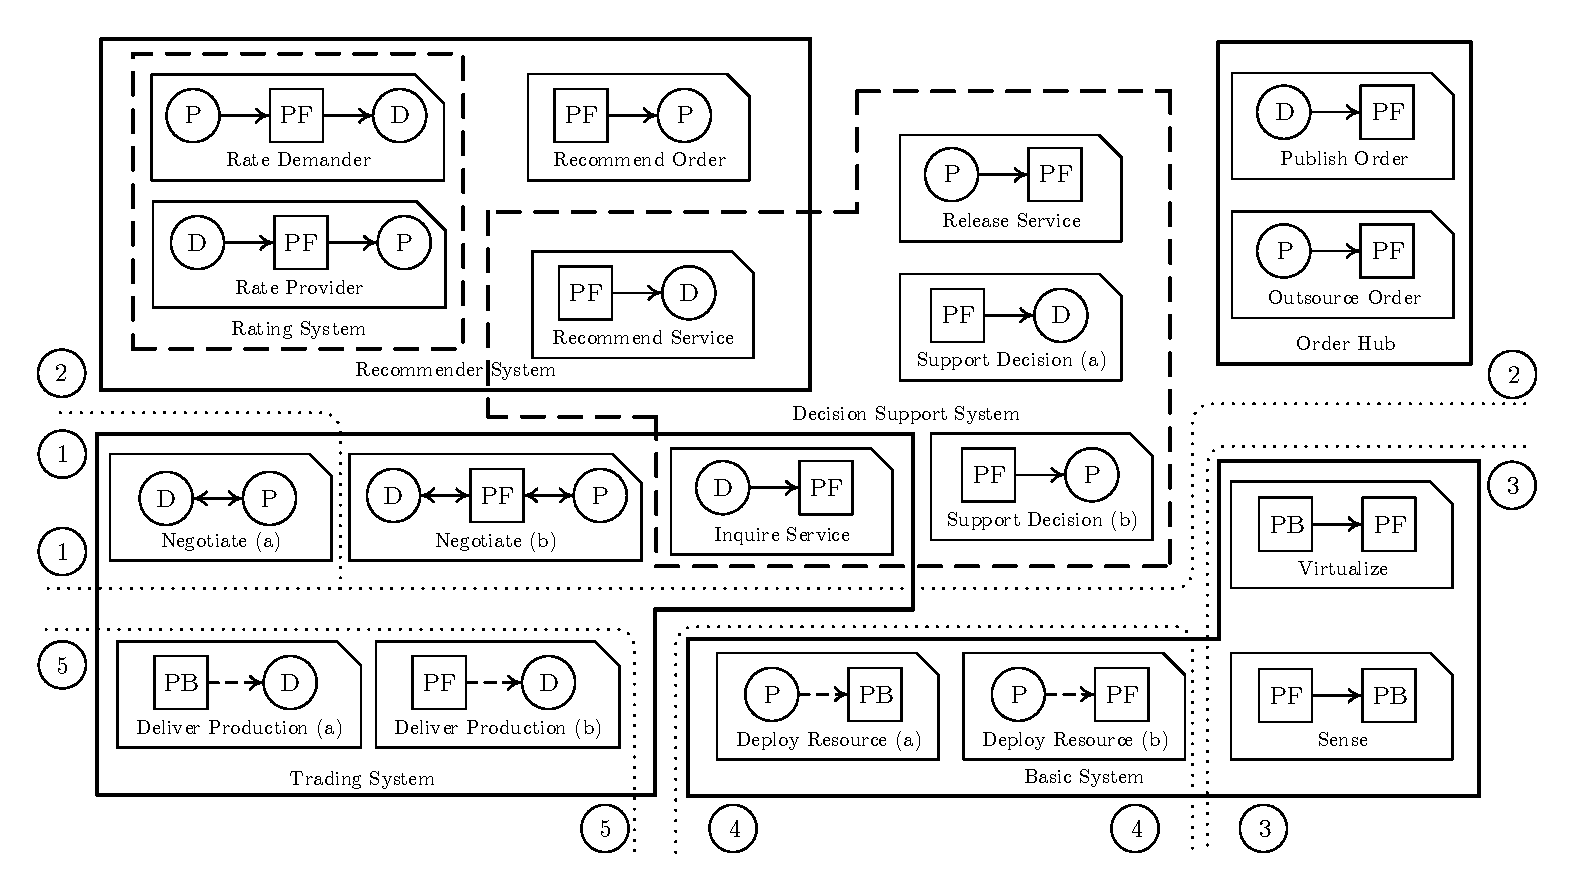
\includegraphics[scale = .6, trim = 0 15 0 10]{supplementary.pdf}
\caption{Supplementay illustration for \autoref{fig:structure}}
\label{fig:supplementary}
\end{figure}

With the supplementary illustration of \autoref{fig:supplementary}, which categorizes the main applications in cloud manufacturing environment with the forementioned flows that marked by circled number (i.e. \textcircled{\small{1}}) and corresponding to the same symbol in \autoref{fig:structure}, we can simply describe the main activities within the cloud manufacturing system. In \autoref{fig:supplementary}, we denote provider, demander, platform and physical base as \textbf{P}, \textbf{D}, \textbf{PF} and \textbf{PB} respectively. The overlap among application districts implies the complexity of the system, so that we will analyse these applications coordinately from a systematic view.

\subsubsection{Operation model}
% 放那两张流程图,以说明流程。分别作为平台及企业自生的运作模式
\begin{figure}[!h]
\centering\small
% \subfloat[Order Flow]{\resizebox{0.45\textwidth}{!}{% !TEX root = flow_head.tex
\begin{tikzpicture}[%
    >=triangle 60,              % Nice arrows; your taste may be different
    start chain=going below,    % General flow is top-to-bottom
    node distance=6mm and 60mm, % Global setup of box spacing
    every join/.style={norm},   % Default linetype for connecting boxes
    ]
% ------------------------------------------------- 
% A few box styles 
% <on chain> *and* <on grid> reduce the need for manual relative
% positioning of nodes
\tikzset{
  base/.style={draw, on chain, on grid, align=center, minimum height=4ex},
  proc/.style={base, rectangle, text width=8em},
  test/.style={base, diamond, aspect=2, text width=5em},
  term/.style={proc, rounded corners},
  % coord node style is used for placing corners of connecting lines
  coord/.style={coordinate, on chain, on grid, node distance=6mm and 25mm},
  % nmark node style is used for coordinate debugging marks
  nmark/.style={draw, cyan, circle, font={\sffamily\bfseries}},
  % -------------------------------------------------
  % Connector line styles for different parts of the diagram
  norm/.style={->, draw, lcnorm},
  free/.style={->, draw, lcfree},
  cong/.style={->, draw, lccong},
  it/.style={font={\small\itshape}}
}
% -------------------------------------------------
% Start by placing the nodes
\node [term] {Be Submitted};
\end{tikzpicture}}\label{fig:orderflow}} \hspace{0.09\textwidth}
% \subfloat[User Rank]{\resizebox{0.45\textwidth}{!}{% !TEX root = flow_head.tex
\begin{tikzpicture}[%
    >=triangle 60,              % Nice arrows; your taste may be different
    start chain=going below,    % General flow is top-to-bottom
    node distance=6mm and 60mm, % Global setup of box spacing
    every join/.style={norm},   % Default linetype for connecting boxes
    ]
% ------------------------------------------------- 
% A few box styles 
% <on chain> *and* <on grid> reduce the need for manual relative
% positioning of nodes
\tikzset{
  base/.style={draw, on chain, on grid, align=center, minimum height=4ex},
  proc/.style={base, rectangle, text width=8em},
  test/.style={base, diamond, aspect=2, text width=5em},
  term/.style={proc, rounded corners},
  % coord node style is used for placing corners of connecting lines
  coord/.style={coordinate, on chain, on grid, node distance=6mm and 25mm},
  % nmark node style is used for coordinate debugging marks
  nmark/.style={draw, cyan, circle, font={\sffamily\bfseries}},
  % -------------------------------------------------
  % Connector line styles for different parts of the diagram
  norm/.style={->, draw, lcnorm},
  free/.style={->, draw, lcfree},
  cong/.style={->, draw, lccong},
  it/.style={font={\small\itshape}}
}
% -------------------------------------------------
% Start by placing the nodes
\node [term]              (m1)  {Be Introduced};
\node [proc, join]        (p8)  {Get Initial Rank $R$};
\node [coord, yshift=2mm] (c1)  {}; \cmark{1}
\node [test, yshift=2mm]  (t1)  {Transact?};
\node [proc, yshift=-3mm] (p1)  {Increase $R$};


\node [proc, right=of t1] (p4)  {Wait};
\node [proc]              (p5)  {Compete to Get Task};
\node [test, join]        (t5)  {Make it?};
\node [coord, yshift=2mm] (c3)  {}; \cmark{3}

\node [test, yshift=2mm]  (t6)  {Outsourcing?};
\node [test]              (t7)  {Partly or Whole?};
\node [proc]              (p6)  {Submit Outsourcing Request};
\node [proc]              (p7)  {Decrease $R$};
\node [test, join]        (t8)  {$R < R_{base}$?};
\node [term]              (m2)  {Eliminate};

\node [test, left=of c3]  (t2)  {All Tasks Accomplished?};
\node [proc]              (p2)  {Process Task};
\node [test]              (t3)  {Accepted?};
\node [proc]              (p3)  {Pass the Outsouring Task};
\node [test]              (t4)  {Task Accomplished?};

\node [coord, left=of p1](c2)  {}; \cmark{2}

\draw [->, lcnorm] (p4) |- (c1);
\draw [->, lcnorm] (p8) -- (t1);
\draw [->, lcnorm] (p1) --(c2) |- (c1);

\path (t1.east)   to node [near start, yshift=1em] {$n$} (p4);
\path (t1.south) to node [near start, xshift=1em] {$y$} (p1);
  \draw [o->, lcnorm] (t1.east) -- (p4);
  \draw [*->, lcnorm] (t1.south) |- (p5);

\end{tikzpicture}}\label{fig:userrank}}
\resizebox{0.9\textwidth}{!}{% !TEX root = ../Eco-Model.tex
\begin{tikzpicture}[%
    >=triangle 60,              % Nice arrows; your taste may be different
    start chain=going right,    % General flow is top-to-bottom
    node distance=6mm and 10mm, % Global setup of box spacing
    every join/.style={norm},   % Default linetype for connecting boxes
    ]
% ------------------------------------------------- 
% A few box styles 
% <on chain> *and* <on grid> reduce the need for manual relative
% positioning of nodes
\tikzset{
  base/.style={draw, on chain, on grid, align=center, rectangle},
  proc/.style={base, text width=6em, minimum height=8em},
  term/.style={base, text width=5em, rounded corners, minimum height = 3ex},
  dproc/.style={proc, minimum height = 20ex},
  gathe/.style={draw, on chain, on grid, align=center, circle, minimum height=4ex, text width=0.5em, node distance=10mm and 8mm},
  % coord node style is used for placing corners of connecting lines
  coord/.style={coordinate, on chain, on grid, node distance=6mm and 25mm},
  sky/.style={coordinate, on chain, on grid, node distance=6mm and 60mm},
  % nmark node style is used for coordinate debugging marks
  nmark/.style={draw, cyan, circle, font={\sffamily\bfseries}},
  % -------------------------------------------------
  % Connector line styles for different parts of the diagram
  norm/.style={->, draw, lcnorm},
  free/.style={->, draw, lcfree},
  cong/.style={->, draw, lccong},
  it/.style={font={\small\itshape}}
}
% -------------------------------------------------
% Start by placing the nodes
\node [term, fill = lcfree!25]              {Order};
\node [proc, join=by free]  (p1) {Task Hub};
\node [proc, dashed] (d) {};
\node [term, xshift = 12mm] (oc) {Order Check};
\node [term, join=by cong, fill = lccong!25]  {Submit};

\node [gathe, right=of d,yshift=5mm, xshift= 15mm] (g1) {};
\node [term, below=of d, yshift=15.5mm] (u1) {User 1};
\node [term, below=of u1] (u2) {User 2};
\node [below=-1mm of u2] (u3) {$\vdots$};
\node [term,below=of u3, yshift=-1mm] (u4) {User n};
\node [below=of u4,yshift=2.6mm] {User Cluster};
\node [gathe, below=of g1] (g2) {};
\node [coord, above=of g1, yshift=8mm] (c1) {};

\draw [->, lccong] (g2) -- (oc.west);
\draw [->, lcnorm] (p1) -- (u1.west);
\draw [->, lcnorm] (p1) -- (u2.west);
\draw [->, lcnorm] (p1) -- (u4.west);

\draw [->, lcnorm] (u1.east) -- (g1.west);
\draw [->, lccong] (u1.east) -- (g2.west);
\draw [->, lcnorm] (u2.east) -- (g1.west);
\draw [->, lccong] (u2.east) -- (g2.west);
\draw [->, lcnorm] (u4.east) -- (g1.west);
\draw [->, lccong] (u4.east) -- (g2.west);
\draw [->, lcnorm] (g1) -- (c1) -- node [black, near end, yshift=0.75em, it]
    {(Outsourcing)} ++(-3.5cm,0) -| (p1) ;

\end{tikzpicture}}
\caption{Simple Flow Chart of Order}
\label{fig:simpleorderflow}
\end{figure}
\subsubsection{Main features in the ecosystem}
% 提一下云制造生态环境中的应用、模块,主要强调这些模块之间的交互,会产生怎样的作用。
As shown in \autoref{fig:structure}, 
Rating system, decision support system, recommender system,
detail info will seen in
Modular approaches are widely used to decompose a complex system into smaller subsystems according to their functions. For example, Yang and Li (2011) divided a cloud manufacturing services management and control platform into seven functional modules such as system management module, production management module and so on

% subsection cloud_manufacturing_ecosystem (end)

\subsection{Main complexity concepts} % (fold)
\label{sub:main_complexity_concepts}

\subsubsection{Self-organization}

\subsubsection{Emergence}

\subsubsection{Co-evolution}

\subsubsection{Adaption}
% subsection main_complexity_concepts (end)

\subsection{Ecosystem evolvement} % (fold)
\label{sub:ecosystem_evolvement}

% subsection ecosystem_evolvement (end)

\subsection{Optimal guidance} % (fold)
\label{sub:optimal_guidance}

% subsection optimal_guidance (end)
% section background (end)